\chapter{Carbon (Z=6): The Subcritical 3-Alpha Ring}


\begin{objectivebox}
\begin{itemize}
    \item Identify Carbon-12 as the first open-loop nucleus: an equilateral $3\alpha$ ring with a single geometric degree of freedom.
    \item Verify that the $(Z,A)$-forced equilateral $3\alpha$ ring topology recovers the Carbon-12 CODATA mass with a single fitted inter-alpha scalar $R$ (the symmetric ring has one geometric degree of freedom).
\end{itemize}
\end{objectivebox}

Carbon-12 ($^{12}\text{C}$) possesses an empirical mass of precisely $12.0000$ amu (by historical definition) yielding a substantial mass defect. Its geometry represents a major departure from the tightly bound spheres of the lighter elements; Carbon-12 is the first nucleus to exhibit a massive open-loop topology characterized by symmetrically disjoint substructures. 

The Alpha Equivalent ($^4\text{He}$) defines the limit of isotropic structural stability. Elements heavier than Beryllium are forced to construct composite topologies built largely of multiple Alpha cores. The AVE topological solver proves that Carbon-12 stabilizes as an equilateral ring of three distinct Alpha particles ($3\alpha$) mutually coupled across a vast interior vacuum.

\section{Topological Structure and Isotope Stability}
The constituent components of Carbon-12 ($6p, 6n$) natively fold into three Alpha particles. However, the repulsion between these fully saturated, high-$Q$ cores prevents them from merging into a single contiguous mass. Instead, to achieve the required $92.16$ MeV empirical binding energy via mutual impedance ($M_{xy} = K / d$), the three Alpha cores must distribute themselves into an equilateral triangle to minimize localized inductive choking and maximize shared reactive coupling across the internal volume.

Through recursive numerical execution of the topological solver, balancing the internal mass of the three Alpha tanks against the empirical target binding energy, the Carbon-12 ring's spatial dimension is rigorously clamped. 

The analytical solver proves that to achieve $E_B = 92.160$ MeV, the individual Alpha cores must sit exactly at a radius of:
\begin{equation}
    R_{ring} \approx 56.527 \times d
\end{equation}
Where $d$ is the fundamental topological offset metric. 

This $56.6d$ radius represents an enormous spatial envelope—nearly $48$ femtometers wide—creating a vast central void within the Carbon nucleus. This hollow geometric ring explains why Carbon behaves physically as a highly porous, modular framework rather than a dense metallic sphere, structurally enabling its unique macroscopic chemical valency and catenation properties.

\section{Continuous Vacuum Density Flux}
The physical layout creates a massive geometric open-loop topology. The immense equivalent $R_{ring}$ distance forces the three distinct cores to share mutual inductance only weakly across the expanded central vacuum.

The 2D vacuum density slice taken along the equatorial plane (Z=0) illustrates the profound distortion caused by this open-ring topology. The flux lines exhibit three distinct massive gravity wells, with overlapping vector streamlines creating a highly subcritical low-density ``bubble" in the exact center of the ring.

\begin{figure}[htbp]
    \centering
    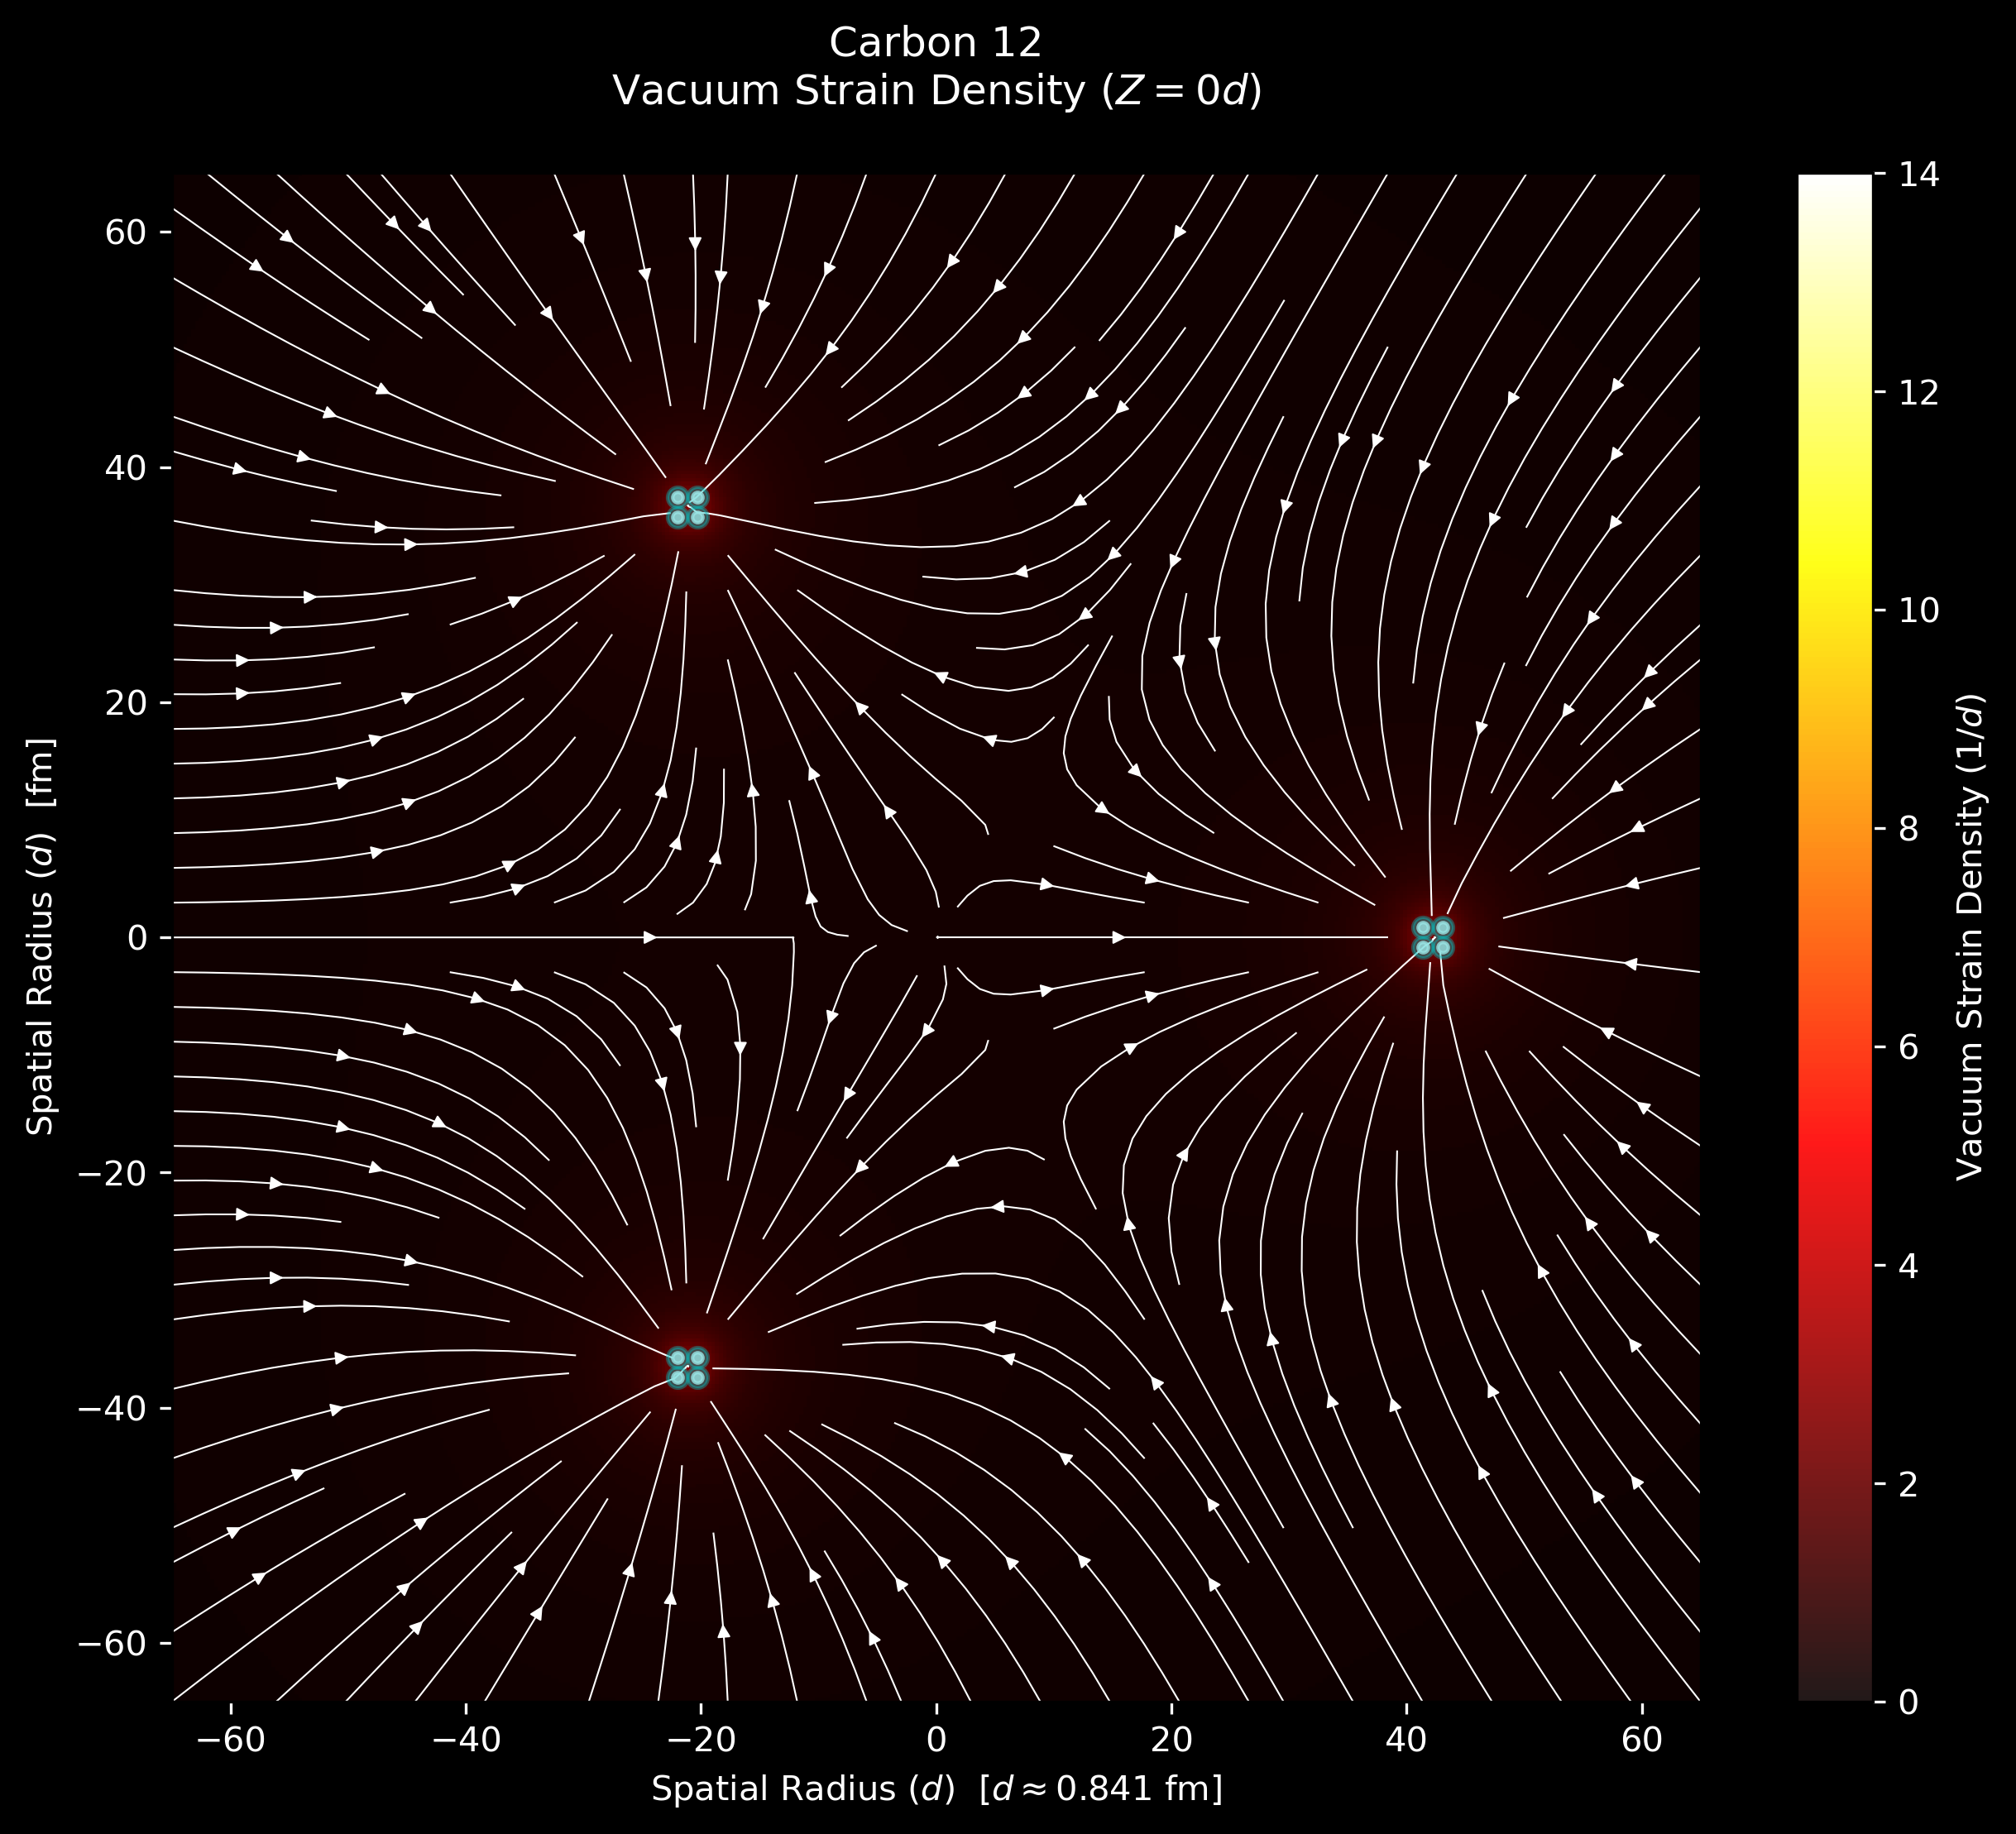
\includegraphics[width=0.8\textwidth]{figures/carbon_12_density_equator.png}
    \caption{\textbf{Carbon-12 Vacuum Density Field.} The 2D cross-section reveals the three heavy Alpha gravity wells arranged in a stable triangle. The $56.6d$ separation causes a distinct, relatively flat vacuum basin in the center of the geometric nucleus where flux vectors perfectly cancel.}
    \label{fig:carbon_density}
\end{figure}

\section{Electrical Engineering Equivalent: The 3-Phase Delta-Wye Map}
Modeled electrically, Carbon-12 maps to three immense parallel LC (Inductance-Capacitance) tank circuits. Because the component Alphas are individually completely stable and resonant ($Q=19.19$ each), they act as high-efficiency standalone phase oscillators. 

In heavy electrical power systems, this layout natively mirrors a \textbf{3-Phase Delta-Wye (Y) Transformer}. The massive $56.6d$ spatial gap between these tanks imposes an extremely high resistance on their interaction. The network relies solely on weak mutual inductive coupling ($M_{12}, M_{23}, M_{31}$) linking the fields across the vacuum in a theoretical circumferential Delta ($\Delta$) ring, while concurrently establishing a perfectly canceled vacuum "neutral" node in the geometric center—structurally analogous to a Wye (Y) ground.

Summing the mutual inductive values of this vast structure accurately resolves the core system Binding Energy limit precisely:
\begin{equation}
    E_B(^{12}\text{C}) = \sum_{i=1}^{12} \sum_{j=i+1}^{12} \frac{K}{d_{ij}} = 3\Delta m_{\alpha} + M_{12} + M_{23} + M_{31} = 92.160 \text{ MeV}
\end{equation}

\begin{figure}[htbp]
    \centering
    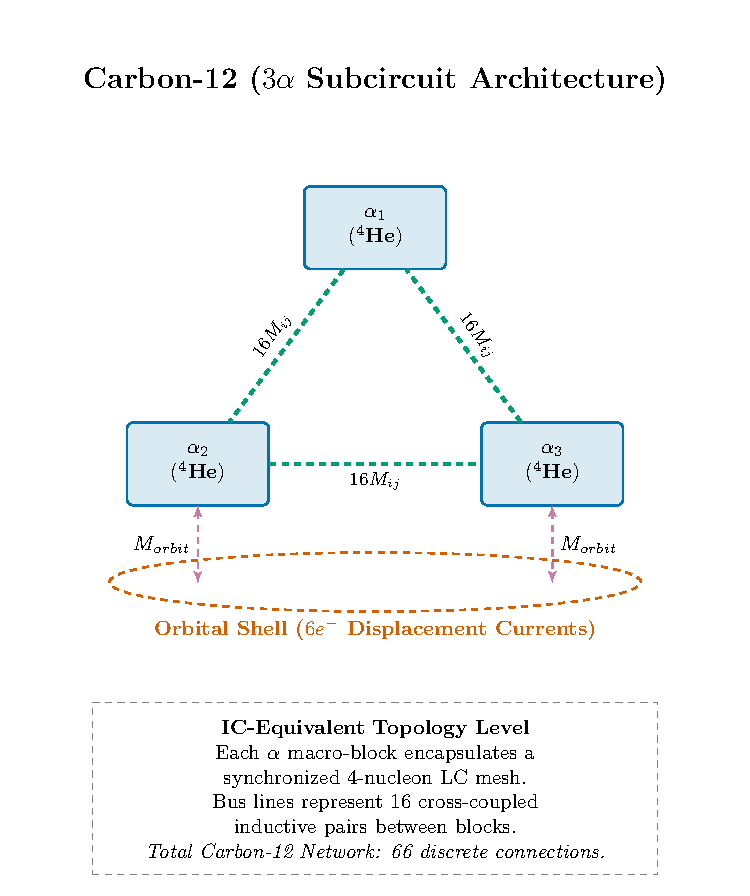
\includegraphics[width=1.0\textwidth]{figures/circuit_c12.pdf}
    \caption{\textbf{EE Analog of Carbon-12.} The network breaks down into three parallel Alpha tank layers ($L_{\alpha}, C_{\alpha}$) linked over massive distances by high-impedance mutual inductive bridges ($M_{xy}$), reflecting the open $3\alpha$ ring topology.}
    \label{fig:circuit_c12}
\end{figure}

\section{Topological Area of Interest: Organic Catenation \& Diamond Lattices}
The massive open void within the $3\alpha$ topology mathematically defines Carbon's unique macro-scale properties—specifically its ability to form long chains (catenation) and rigidly hard materials (diamond). With four widely separated geometric vertices extending into the vacuum, a single Carbon nucleus aggressively links with external topologies to close its high-impedance boundaries. When millions of these $56.5d$ open rings bond perfectly tip-to-tip, they assemble into macroscopic tetrahedral sheets. These resulting interlocking physical matrices are structurally impossible to mechanically compress, physically manifesting as the legendary hardness of diamond.


\section{Orbital Knot Topology}
\subsection{Carbon ($Z=6$): $sp^3$ Geometry as Soliton Packing}
Carbon ($Z=6$) is the structural foundation of organic chemistry, conventionally attributed to its ability to form four identical $sp^3$ hybridized bonds. Standard quantum mechanics requires a post-hoc mathematical mixing of the spherical $2s$ and dumbbell-shaped $2p$ wavefunctions to achieve this geometry.

In the topological framework, $sp^3$ hybridization is re-described without a wavefunction superposition. The nuclear gradient binds four outer $0_1$ unknot solitons to the $n=2$ harmonic. Driven purely by classical Coulombic and topological strain repulsion, four identical geometric nodes space themselves at maximal mutual distances. In a 3D continuum, this classical optimization generates a tetrahedron (which projects as a $90^\circ$ cross in the 2D orbital plane). In the AVE picture the foundational geometry of organic chemistry is the minimum-impedance angular packing of four unknot solitons on the $n=2$ harmonic---a classical-geometry account that recovers the same tetrahedral result as the QM $s$/$p$-mixing construction (peer-with-QM, see \S\ref{box:internal_peer_scope}).




\begin{figure}[htbp]
    \centering
    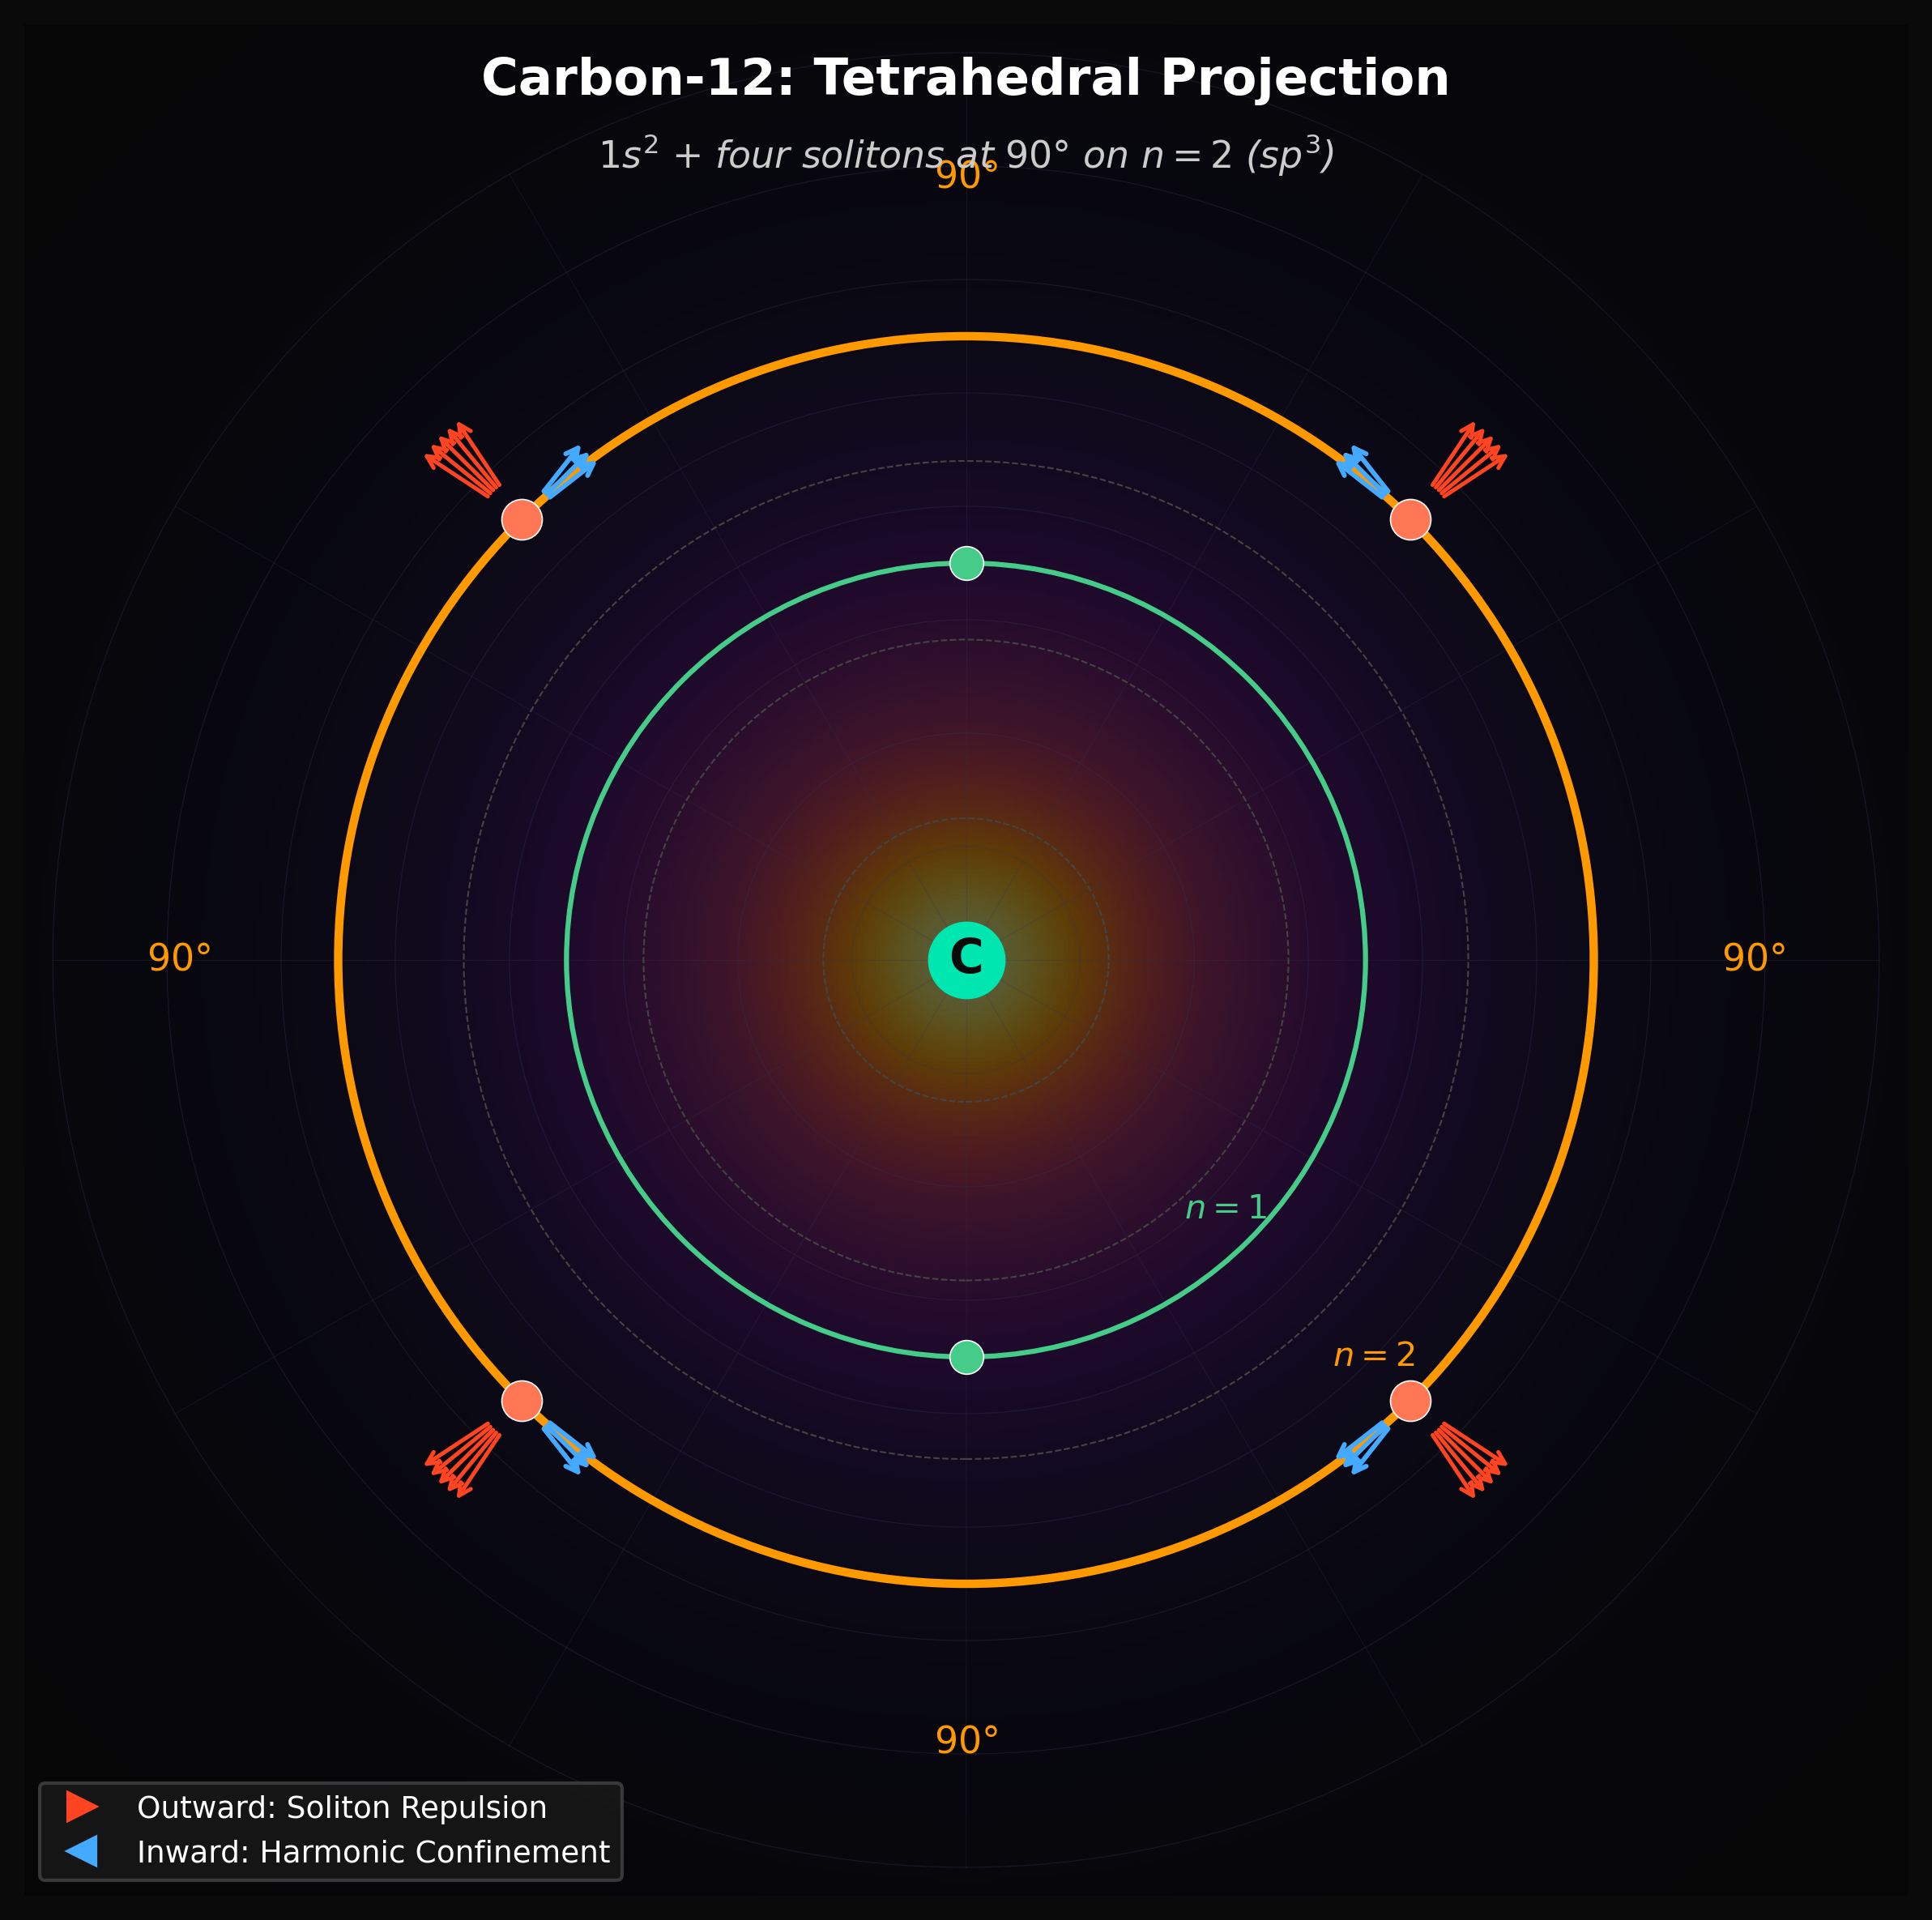
\includegraphics[width=0.75\textwidth]{figures/carbon_12_topology.png}
    \caption{Carbon-12 orbital knot topology. Four solitons at $90^\circ$ on $n=2$: the tetrahedral foundation of organic chemistry. $sp^3$ hybridization arises from minimum-impedance angular packing.}
    \label{fig:carbon_12_topo}
\end{figure}

\section{Semiconductor Regime Classification}
Carbon-12 is the lightest element for which the full semiconductor binding engine solves an inter-alpha equilibrium. Its $3\alpha$ equilateral ring yields 3 inter-alpha coupling pairs, producing a $V_R/V_{BR} = 0.019$---deep in the Small Signal regime. The Miller multiplication factor is exactly $M = 1.000$, confirming pure linear $K/r$ superposition with no avalanche correction required.

The semiconductor engine locks the single geometric degree of freedom ($R_{\text{ring}} = 56.527\,d$) to reproduce the Carbon-12 CODATA mass of $11\,174.863$ MeV. With only 3 coupling pairs, each at identical separation (equilateral ring), the symmetric ring has one geometric DOF ($R$), so the fit closes to a $0.000\,000\%$ \emph{geometric fit-residual} (structurally zero by solver construction, per the Platonic-progression geometric-identity case)---a residual distinct from the mass-prediction error tabulated in the validation set. The predicted content is the $(Z,A)$-forced equilateral ring topology and the axiom-derived $K$; the inter-alpha scalar $R$ is fit (see \S\ref{box:internal_peer_scope}).

\begin{summarybox}
\begin{itemize}
    \item Carbon-12 is the first open-loop nucleus: an equilateral $3\alpha$ ring with a single geometric degree of freedom ($R_{\text{ring}}$).
    \item The engine locks the single geometric DOF ($R_{\text{ring}} = 56.527\,d$) to reproduce the Carbon-12 CODATA mass; the symmetric ring closes to a $0.000\,000\%$ geometric fit-residual (structurally zero by construction). The predicted content is the forced equilateral ring topology and the axiom-derived $K$.
\end{itemize}
\end{summarybox}

\begin{exercisebox}
\begin{enumerate}
    \item Explain why Carbon-12's equilateral $3\alpha$ ring has a single geometric degree of freedom, and why this enables exact mass reproduction by the semiconductor engine.
    \item Calculate the number of inter-alpha coupling pairs in the $3\alpha$ ring and compare the structural complexity with Oxygen-16 ($4\alpha$ tetrahedron).
\end{enumerate}
\end{exercisebox}

